\documentclass[ngerman]{article}
\usepackage[T1]{fontenc}
\usepackage[latin9]{inputenc}
\usepackage[letterpaper]{geometry}
\geometry{verbose,tmargin=3cm,bmargin=3cm,lmargin=3cm,rmargin=3cm}
\usepackage{babel}
\usepackage{graphicx}
%Packages f�r eigen definierte Header und Footer
\usepackage{lastpage}
\usepackage{fancyhdr}

% doctitel = Titel des Dokuments
% docvers = Versionsnr.
% docautor = Author(en)
% docdate = Datum der letzten �nderung
\def\doctitel{Dokumententitel}
\def\docvers{1.0}
\def\docautor{Max Mustermann}
\def\docdate{12. Juli 2009}

% docstate = Status des Dokuments aus {neu, bearbeitet}
% qsstate = QS-Pr�fungsstatus aus {positiv QS-gepr�ft, negativ QS-gepr�ft, verworfen}
% proofstate = Pr�fungsstatus (durch Projektleiter) aus {positiv gepr�ft, negativ gepr�ft, verworfen}
% reviewstate = Annahmestatus des Reviews {kein Review durchgef�hrt, akzeptiert ohne �nderungen, akzeptiert mit �nderungen, nicht akzeptiert}
% endstate = Endstatus des Dokuments aus {freigegeben, verworfen}
\def\docstate{neu}
\def\qsstate{nicht QS-gepr�ft}
\def\proofstate{nicht gepr�ft}
\def\reviewstate{kein Review durchgef�hrt}
\def\endstate{-}

%Nicht einr�cken
%\setlength{\parindent}{0pt}

\begin{document}

%Header und Footer Definitionen f�r das Deckblatt
\thispagestyle{fancy}
\renewcommand{\headrulewidth}{0mm}
\lhead{{\small }}
\chead{{\small }}
\rhead{{\small }}
\lfoot{{\small SIMPL � 2009 \$IMPL}}
\cfoot{{\small \docdate}}
\rfoot{{\small \thepage\ / \pageref{LastPage}}}


%Text f�r das Deckblatt
\vspace*{5cm}
\noindent{\LARGE Studienprojekt SIMPL} \\
\noindent\rule[1ex]{\textwidth}{1pt}
\vspace*{1cm}
\begin{flushleft}
	{\Huge \textbf{\doctitel}} \\
	\vspace{0.5cm}
	{\LARGE Version \docvers} \\
	\vspace{0.5cm}
	{\LARGE \docdate} \\
	\vspace{0.5cm}
	{\LARGE Verfasser: \docautor}
\end{flushleft}
\vspace*{1cm}
\noindent\rule[1ex]{\textwidth}{1pt}

\vspace*{2cm}
\begin{center}
	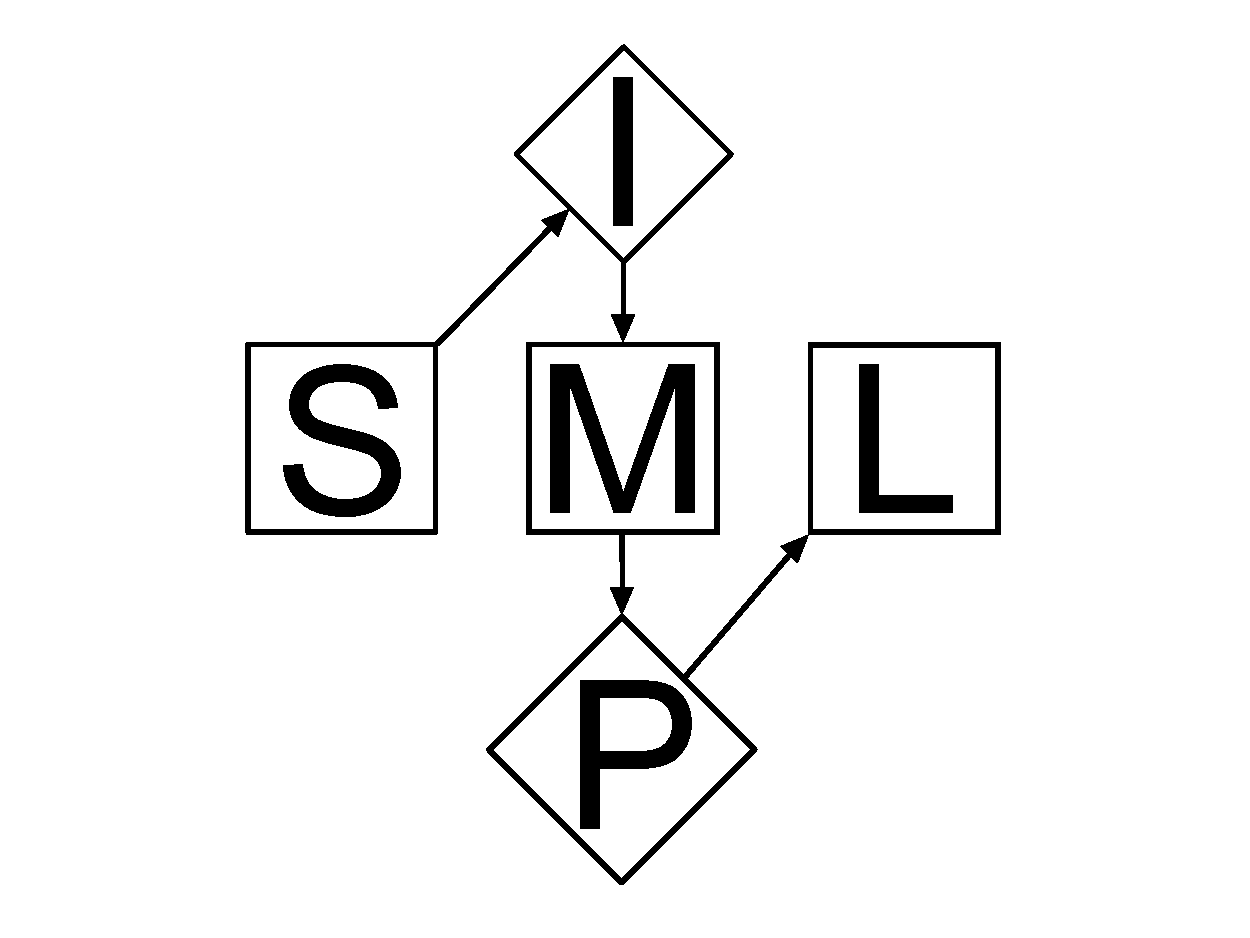
\includegraphics{SIMPL}
\end{center}

%Neue Seite beginnen
\pagebreak{}

%Header und Footer Definitionen f�r das Deckblatt
\thispagestyle{fancy}
\renewcommand{\headrulewidth}{0mm}
\lhead{{\small }}
\chead{{\small }}
\rhead{{\small }}
\lfoot{{\small SIMPL � 2009 \$IMPL}}
\cfoot{{\small \docdate}}
\rfoot{{\small \thepage\ / \pageref{LastPage}}}


%Text f�r das Deckblatt
\vspace*{5cm}
\noindent{\LARGE Studienprojekt SIMPL} \\
\noindent\rule[1ex]{\textwidth}{1pt}
\vspace*{1cm}
\begin{flushleft}
	{\Huge \textbf{Dok-Status:} \docstate} \\
	\vspace{0.5cm}
	{\Huge \textbf{QS-Status:} \qsstate} \\
	\vspace{0.5cm}
	{\Huge \textbf{Pr�f-Status:} \proofstate} \\
	\vspace{0.5cm}
	{\Huge \textbf{End-Status:} \endstate}
\end{flushleft}
\vspace*{1cm}
\noindent\rule[1ex]{\textwidth}{1pt}

%Neue Seite beginnen
\pagebreak{}

%Header und Footer Definitionen f�r alle anderen Seiten
\pagestyle{fancy}
\renewcommand{\headrulewidth}{0mm}
\lhead{{\small }}
\chead{{\small }}
\rhead{{\small }}
\lfoot{{\small SIMPL � 2009 \$IMPL}}
\cfoot{{\small }}
\rfoot{{\small \thepage\ / \pageref{LastPage}}}

%Ab hier beginnt das Dokument
\tableofcontents

\newpage{}

\section{�nderungsgeschichte}
\begin{itemize}
\item \textbf{Version 0.1}, 22. Juni 2009: Erstellung des Dokuments.
\end{itemize}

\end{document}
